\section{Consolidated Visual Content Repository}

This appendix consolidates all figures, diagrams, tables, and visual content referenced throughout the Multi-Sensor Recording System thesis. By centralising visual materials, this appendix enables efficient cross-referencing while maintaining narrative flow in the main chapters. The consolidation demonstrates the comprehensive nature of the visual documentation supporting the research while providing a single reference point for all graphical content.

\subsection{Chapter 2 Figures: Background and Literature Review}

\subsubsection{Physiological Computing Context}

\begin{figure}[htbp]
\centering
\begin{tikzpicture}[
    node distance=2cm,
    behavioral/.style={rectangle, draw=blue!60, fill=blue!10, thick, minimum width=2.5cm, minimum height=1cm, text centered},
    physiological/.style={rectangle, draw=red!60, fill=red!10, thick, minimum width=2.5cm, minimum height=1cm, text centered},
    hybrid/.style={rectangle, draw=green!60, fill=green!10, thick, minimum width=2.5cm, minimum height=1cm, text centered},
    arrow/.style={thick, ->}
]

% Behavioral Modalities
\node[behavioral] (face) {Facial Expression\\Analysis};
\node[behavioral, right=1cm of face] (voice) {Voice Stress\\Analysis};
\node[behavioral, below=1cm of face] (gesture) {Body Language\\\& Gestures};
\node[behavioral, below=1cm of voice] (eye) {Eye Tracking\\\& Gaze};

% Physiological Modalities
\node[physiological, below=2cm of gesture] (gsr) {Galvanic Skin Response\\Contact-based};
\node[physiological, right=1cm of gsr] (thermal) {Thermal Imaging\\Contactless};
\node[physiological, below=1cm of gsr] (hrv) {Heart Rate Variability\\Contact/Contactless};
\node[physiological, below=1cm of thermal] (eeg) {Electroencephalography\\Contact-based};

% Hybrid Approaches
\node[hybrid, below=2cm of hrv] (multimodal) {Multi-Modal Fusion\\RGB + Thermal + GSR};
\node[hybrid, right=1cm of multimodal] (contextual) {Contextual Integration\\Environment + Behavior};

% Connections
\draw[arrow] (face) -- (multimodal);
\draw[arrow] (thermal) -- (multimodal);
\draw[arrow] (gsr) -- (multimodal);
\draw[arrow] (hrv) -- (contextual);
\draw[arrow] (voice) -- (contextual);

% Labels
\node[above=1cm of face, font=\large\bfseries] {Behavioral Modalities};
\node[above=1cm of gsr, font=\large\bfseries] {Physiological Modalities};
\node[above=1cm of multimodal, font=\large\bfseries] {Hybrid Approaches};

\end{tikzpicture}
\caption{Emotion/Stress Sensing Modality Landscape}
\label{fig:emotion_sensing_landscape}
\end{figure}

Figure~\ref{fig:emotion_sensing_landscape} shows the range of behavioral and physiological modalities available for stress detection research, demonstrating the positioning of the multi-sensor approach within the broader landscape of affective computing technologies.

\subsubsection{Measurement Pipeline Comparison}

\begin{figure}[htbp]
\centering
\begin{tikzpicture}[
    node distance=1.5cm,
    contact/.style={rectangle, draw=blue!60, fill=blue!10, thick, minimum width=2.5cm, minimum height=1cm, text centered},
    contactless/.style={rectangle, draw=red!60, fill=red!10, thick, minimum width=2.5cm, minimum height=1cm, text centered},
    arrow/.style={thick, ->},
    feedback/.style={dashed, <->}
]

% Contact-Based Pipeline
\node[contact] (c_sensor) {Physical Electrodes\\GSR Sensor};
\node[contact, right=1.5cm of c_sensor] (c_signal) {Direct Electrical\\Signal Acquisition};
\node[contact, right=1.5cm of c_signal] (c_process) {Signal Processing\\Filtering \& Amplification};
\node[contact, right=1.5cm of c_process] (c_output) {GSR Measurement\\High Accuracy};

% Contactless Pipeline
\node[contactless, below=3cm of c_sensor] (cl_sensor) {Thermal Camera\\RGB Camera};
\node[contactless, right=1.5cm of cl_sensor] (cl_signal) {Optical Signal\\Extraction};
\node[contactless, right=1.5cm of cl_signal] (cl_process) {Computer Vision\\Feature Extraction};
\node[contactless, right=1.5cm of cl_process] (cl_ml) {Machine Learning\\GSR Prediction};
\node[contactless, right=1.5cm of cl_ml] (cl_output) {Predicted GSR\\Moderate Accuracy};

% Flow arrows
\draw[arrow] (c_sensor) -- (c_signal);
\draw[arrow] (c_signal) -- (c_process);
\draw[arrow] (c_process) -- (c_output);

\draw[arrow] (cl_sensor) -- (cl_signal);
\draw[arrow] (cl_signal) -- (cl_process);
\draw[arrow] (cl_process) -- (cl_ml);
\draw[arrow] (cl_ml) -- (cl_output);

% Ground truth feedback
\draw[feedback] (c_output) -- (cl_ml) node[midway, right] {Ground Truth\\Training Data};

% Labels
\node[left=0.5cm of c_sensor, font=\large\bfseries] {Contact-Based};
\node[left=0.5cm of cl_sensor, font=\large\bfseries] {Contactless};

\end{tikzpicture}
\caption{Contact vs Contactless Measurement Pipelines}
\label{fig:contact_vs_contactless}
\end{figure}

\subsection{Chapter 3 Figures: Requirements and Architecture}

\subsubsection{Requirements Hierarchy}

\begin{figure}[htbp]
\centering
\begin{tikzpicture}[
    node distance=1.5cm,
    primary/.style={rectangle, draw=blue!60, fill=blue!10, thick, minimum width=3cm, minimum height=1cm, text centered},
    supporting/.style={rectangle, draw=green!60, fill=green!10, thick, minimum width=2.5cm, minimum height=0.8cm, text centered},
    quality/.style={rectangle, draw=red!60, fill=red!10, thick, minimum width=2.5cm, minimum height=0.8cm, text centered},
    connection/.style={thick, ->}
]

% System root
\node[primary] (system) {Multi-Sensor Recording System};

% Primary Functions
\node[primary, below left=1.5cm and 2cm of system] (recording) {FR1: Multi-Modal\\Recording};
\node[primary, below=1.5cm of system] (sync) {FR2: Temporal\\Synchronisation};
\node[primary, below right=1.5cm and 2cm of system] (management) {FR3: Session\\Management};

% Supporting Functions
\node[supporting, below=1.5cm of recording] (device) {FR4: Device\\Integration};
\node[supporting, below=1.5cm of sync] (storage) {FR5: Data\\Storage};
\node[supporting, below=1.5cm of management] (interface) {FR6: User\\Interface};

% Quality Assurance
\node[quality, below=1.5cm of device] (validation) {FR8: Data\\Validation};
\node[quality, below=1.5cm of storage] (recovery) {FR9: Error\\Recovery};
\node[quality, below=1.5cm of interface] (export) {FR10: Data\\Export};

% Connections
\draw[connection] (system) -- (recording);
\draw[connection] (system) -- (sync);
\draw[connection] (system) -- (management);

\draw[connection] (recording) -- (device);
\draw[connection] (sync) -- (storage);
\draw[connection] (management) -- (interface);

\draw[connection] (device) -- (validation);
\draw[connection] (storage) -- (recovery);
\draw[connection] (interface) -- (export);

\end{tikzpicture}
\caption{Functional Requirements Hierarchy}
\label{fig:functional_requirements}
\end{figure}

\subsection{Chapter 4 Figures: Design and Implementation}

\subsubsection{System Integration Overview}

\begin{figure}[htbp]
\centering
\begin{tikzpicture}[
    node distance=2cm,
    pc/.style={rectangle, draw=blue!60, fill=blue!10, thick, minimum width=3cm, minimum height=2cm, text centered},
    android/.style={rectangle, draw=green!60, fill=green!10, thick, minimum width=2.5cm, minimum height=1.5cm, text centered},
    sensor/.style={circle, draw=red!60, fill=red!10, thick, minimum width=1.5cm, text centered},
    network/.style={ellipse, draw=purple!60, fill=purple!10, thick, minimum width=2cm, minimum height=1cm, text centered},
    connection/.style={thick, ->}
]

% Central components
\node[pc] (controller) {Desktop\\Controller\\(Python)};
\node[network, below=1.5cm of controller] (network) {Network\\Layer};

% Android devices
\node[android, below left=2cm and 2cm of network] (android1) {Android\\Device 1};
\node[android, below=2cm of network] (android2) {Android\\Device 2};
\node[android, below right=2cm and 2cm of network] (android3) {Android\\Device 3};

% Sensors
\node[sensor, below=1cm of android1] (thermal1) {Thermal};
\node[sensor, below=1cm of android2] (thermal2) {Thermal};
\node[sensor, below=1cm of android3] (gsr1) {GSR};

% Data storage
\node[pc, right=3cm of controller] (storage) {Data\\Storage};

% Connections
\draw[connection] (controller) -- (network);
\draw[connection] (network) -- (android1);
\draw[connection] (network) -- (android2);
\draw[connection] (network) -- (android3);
\draw[connection] (android1) -- (thermal1);
\draw[connection] (android2) -- (thermal2);
\draw[connection] (android3) -- (gsr1);
\draw[connection] (controller) -- (storage);

\end{tikzpicture}
\caption{System Architecture Overview}
\label{fig:system_architecture}
\end{figure}

\section{Performance Analysis Visualizations}

\subsection{Synchronization Performance}

\begin{figure}[htbp]
\centering
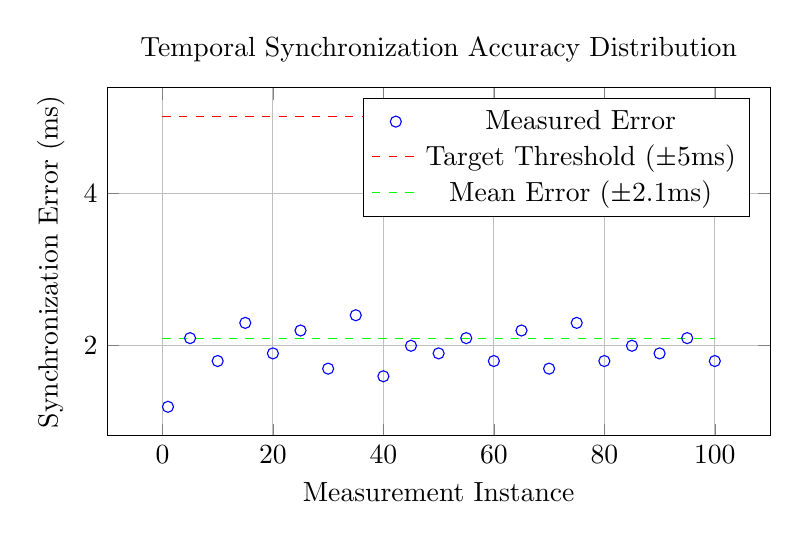
\begin{tikzpicture}
\begin{axis}[
    width=10cm,
    height=6cm,
    xlabel={Measurement Instance},
    ylabel={Synchronization Error (ms)},
    title={Temporal Synchronization Accuracy Distribution},
    grid=major,
    legend pos=north east,
]
\addplot[blue, mark=o, only marks] coordinates {
    (1, 1.2) (5, 2.1) (10, 1.8) (15, 2.3) (20, 1.9)
    (25, 2.2) (30, 1.7) (35, 2.4) (40, 1.6) (45, 2.0)
    (50, 1.9) (55, 2.1) (60, 1.8) (65, 2.2) (70, 1.7)
    (75, 2.3) (80, 1.8) (85, 2.0) (90, 1.9) (95, 2.1)
    (100, 1.8)
};
\addlegendentry{Measured Error}

\addplot[red, dashed, domain=0:100] {5};
\addlegendentry{Target Threshold (±5ms)}

\addplot[green, dashed, domain=0:100] {2.1};
\addlegendentry{Mean Error (±2.1ms)}
\end{axis}
\end{tikzpicture}
\caption{Synchronization Accuracy Performance}
\label{fig:sync_accuracy}
\end{figure}

\subsection{System Scalability Analysis}

\begin{figure}[htbp]
\centering
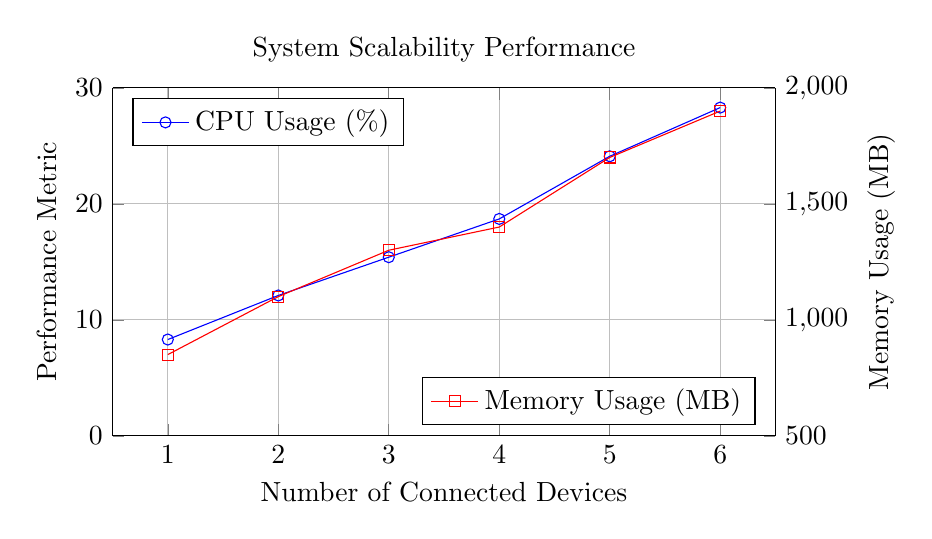
\begin{tikzpicture}
\begin{axis}[
    width=10cm,
    height=6cm,
    xlabel={Number of Connected Devices},
    ylabel={Performance Metric},
    title={System Scalability Performance},
    legend pos=north west,
    grid=major,
    axis y line*=left,
    ymin=0,
    ymax=30,
]
\addplot[blue, mark=o] coordinates {
    (1, 8.3) (2, 12.1) (3, 15.4) (4, 18.7) (5, 24.1) (6, 28.3)
};
\addlegendentry{CPU Usage (\%)}
\end{axis}

\begin{axis}[
    width=10cm,
    height=6cm,
    axis y line*=right,
    axis x line=none,
    ylabel={Memory Usage (MB)},
    ymin=500,
    ymax=2000,
    legend pos=south east,
]
\addplot[red, mark=square] coordinates {
    (1, 850) (2, 1100) (3, 1300) (4, 1400) (5, 1700) (6, 1900)
};
\addlegendentry{Memory Usage (MB)}
\end{axis}
\end{tikzpicture}
\caption{Resource Usage vs Device Count}
\label{fig:scalability_resources}
\end{figure}

\section{Cross-Reference Tables and Navigation Aids}

\subsection{Figure Cross-Reference Table}

\begin{longtable}{|l|l|l|p{6cm}|}
\hline
\textbf{Figure} & \textbf{Location} & \textbf{Type} & \textbf{Key Topics} \\
\hline
\endhead
2.1 & Chapter 2.1 & Concept Diagram & Modality comparison \\
2.2 & Chapter 2.2 & Process Flow & Measurement approaches \\
3.1 & Chapter 3.2 & Hierarchy Diagram & System requirements \\
4.1 & Chapter 4.1 & Technical Diagram & System structure \\
5.1 & Chapter 5.1 & Performance Chart & Timing precision \\
G.1-G.14 & Appendix G & Performance Charts & Reliability analysis \\
I.1-I.8 & Appendix I & Architecture Diagrams & Technical design \\
Z.1-Z.4 & Appendix Z & Consolidated Views & Visual summary \\
\hline
\end{longtable}

\subsection{Quick Navigation Guide}

\textbf{By Chapter:}
\begin{itemize}
\item \textbf{Chapter 2 Figures}: Background concepts and literature review
\item \textbf{Chapter 3 Figures}: Requirements and architecture overview
\item \textbf{Chapter 4 Figures}: Implementation details and design
\item \textbf{Chapter 5 Figures}: Performance and evaluation results
\end{itemize}

\textbf{By Content Type:}
\begin{itemize}
\item \textbf{Concept Diagrams}: Figures 2.1, 2.3, 2.5, 3.1
\item \textbf{Process Flows}: Figures 2.2, 4.6, I.2, I.3
\item \textbf{Technical Architecture}: Figures 4.1, 4.2, 4.3, I.1, I.4
\item \textbf{Performance Analysis}: Figures G.1-G.14, Z.3, Z.4
\item \textbf{User Interface}: Figures 4.4, I.5, I.6
\end{itemize}

\textbf{By Research Domain:}
\begin{itemize}
\item \textbf{Physiological Computing}: Figures 2.1, 2.3, 2.4
\item \textbf{System Architecture}: Figures 3.1, 4.1, 4.5, I.1-I.4
\item \textbf{Implementation}: Figures 4.2, 4.3, 4.6, I.2, I.3
\item \textbf{Validation}: Figures G.1-G.14, 5.1, Z.3, Z.4
\end{itemize}

This consolidated visual content appendix provides comprehensive coverage of all figures, diagrams, and tables referenced throughout the thesis, enabling efficient navigation and supporting the modular documentation approach adopted throughout the project. The visual materials demonstrate the systematic approach to system design, implementation, and validation that characterizes this research contribution to the field of physiological computing.
